%% (c) 2012 florian jung
%% we should consider putting this under a proper license. GPL, or
%% some GPL-like documentation license??

%% rules for editing documentation: (READ THIS FIRST)
%% ~~~~~~~~~~~~~~~~~~~~~~~~~~~~~~~~~~~~~~~~~~~~~~~~~~
%%
%% please try to let newly written lines be shorter than 72 characters.
%% minor exceptions are okay, but please not more than 80 chars.
%% comments shall start after character #80 of the line (that is,
%% they shall be "on the right margin")
%%
%% DON'T MIX up changes and reformatting in one commit. when changing
%% stuff, please don't touch the lines before and after your change
%% (that is, do not re-wrap them), even if it will look a bit patchy.
%% this is for being able to easily use diff.
%% when you want to reformat this file, then do it. but don't change
%% anything, as this would be hard to find in a diff. and clearly
%% state in the commit log that you "only" rearranged things.
%%
%% please adhere to the "User's manual" / "Internals" / "Design"
%% partitioning (genereally, don't change the chapters until there
%% is a really good reason for doing so (adding a chapter like
%% "feature requests" as flo did in r1497 IS one).
%% Below that, feel free to change the logical arrangement
%% (making paragraphs to subsections and similar) if you deem it
%% neccessary.
%%
%% Whenever referring to code symbols, constants or source/header
%% files, please use \sym{someClass::someSymbol}, \usym{UPPERCASE_THING}
%% or \f{file.cpp}.
%% Only specify file paths or namespaces where it would be ambiguous
%% otherwise. Specify 'someClass::' until it would disturb the reader
%% and it is obvious. you have to replace '_' by {\_} (with the {}!).
%% These macros do automatic hyphenation on Camel-Case, under_-score
%% and scope::-operator boundaries. If you need to insert additional
%% hyphenation points, use {\-}.
%% Example: \sym{someClass::someAb{\-}nor{\-}mal{\-}lyLongName} will
%%          hyphenate: some-Class::-some-Ab-nor-mal-ly-Long-Name
%%
%% Whenever referring to URLs, please wrap them in \url{blah}. Key
%% combinations shall look like \key{CTRL+C}. Menu items shall look
%% like \menu{Menu > Submenu > Menu Item}.
%%
%% Where possible, reference other parts of this documents with
%% \label and \ref. Avoid duplicate information under "Internals" by
%% referring to the appropriate section in "User's manual".
%%
%% Please do no time-stamping of sections. if you need time-stamps,
%% use "svn blame documentation.tex"
%%
%% If you contribute something, feel free to add yourself to \author.
%%
%% If you don't speak LaTeX fluently, a few tips:
%% * \section, \subsection, \subsubsection, \paragraph, \subparagraph
%%   let you create sections etc. just copy-and-paste if unsure.
%% * you must prefix special characters like the underscore with \
%%   (backslash)
%% * \emph{some text} emphasizes the text, printing it italic.
%% * \texttt{some text} displays the text in a typewriter font
%% * \label{someName} creates a label at this position. this doesn't
%%   show up in the pdf. with \ref{someName}, you can reference to this
%%   label. (LaTeX will insert the section number instead of \ref)
%%   For this to work, you might need to recompile the .tex twice.
%%
%%%%%%%%%%%%%%%%%%%%%%%%%%%%%%%%%%%%%%%%%%%%%%%%%%%%%%%%%%%%%%%%%%%%%%%%



\documentclass[a4paper]{report}
\usepackage[a4paper,  left=2.5cm, right=2.5cm, top=2.5cm, bottom=2.5cm]{geometry}
\usepackage[T1]{fontenc}
\usepackage[utf8]{inputenc}
\usepackage{lmodern}
\usepackage[english]{babel}
\usepackage{graphicx}
\usepackage{hyphenat}
\usepackage{wrapfig}
\usepackage{fancyhdr}
\pagestyle{fancy}
	\lhead{\scriptsize{\slshape\leftmark}}
	\chead{}
	\rhead{\thepage}
	\lfoot{}
	\cfoot{}
	\rfoot{}
	\renewcommand{\headrulewidth}{0.4pt}
\usepackage{ifthen}

% Hyphenate symbols before each uppercase letter, after each underscore
% (without a "-") and after each ':' (without a "-")
% TODO for any latex crack: also do automatic hyphenation, that is,
% instead of some-Automation-Expression, do some-Au-to-ma-tion-Ex-press-ion
\makeatletter
\newcommand{\camelhyph}[1]{\@fterfirst\c@amelhyph#1\relax }
\newcommand{\underscorehyph}[1]{\@fterfirst\u@nderscorehyph#1\relax }
\def\@fterfirst #1#2{#2#1}
\def\c@amelhyph #1{%
\ifthenelse{\equal{#1}\relax}{}{%  Do nothing if the end has been reached
  \ifnum`#1=95 \_\hspace{0pt}\else      %     Check whether #1 is "_", then print _[thin space]
    \ifnum`#1=58 :\hspace{0pt}\else
      \ifnum`#1>64
        \ifnum`#1<91 \-#1\else#1\fi%     Check whether #1 is an uppercase letter,
      \else#1\fi
    \fi
  \fi
                            %     if so, print \-#1, otherwise #1
  \expandafter\c@amelhyph%    %     insert \c@amelhyph again.
}}
\def\u@nderscorehyph #1{%
\ifthenelse{\equal{#1}\relax}{}{%  Do nothing if the end has been reached
  \ifnum`#1=95 \_\hspace{0pt}\else      %     Check whether #1 is "_", then print _\-
    \ifnum`#1=58 :\hspace{0pt}\else#1\fi\fi
  \expandafter\u@nderscorehyph%    %     insert \u@nderscorehyph again.
}}
\makeatother



\author{Florian Jung, Robert Jonsson}
\title{MusE Documentation}

\newcommand{\url}[1]{\texttt{#1}}
\newcommand{\key}[1]{\textbf{#1}}
\newcommand{\shell}[1]{\texttt{\textbf{#1}}}
\newcommand{\menu}[1]{\textbf{#1}}
\newcommand{\sym}[1]{\texttt{\camelhyph{#1}}}
\newcommand{\usym}[1]{\texttt{\underscorehyph{#1}}}
\newcommand{\file}[1]{\texttt{\camelhyph{#1}}}
\newcommand{\screenshotwidth}[0]{0.8\textwidth}


\begin{document}
\label{Main/Arranger}
\begin{figure}[htp]
\centering
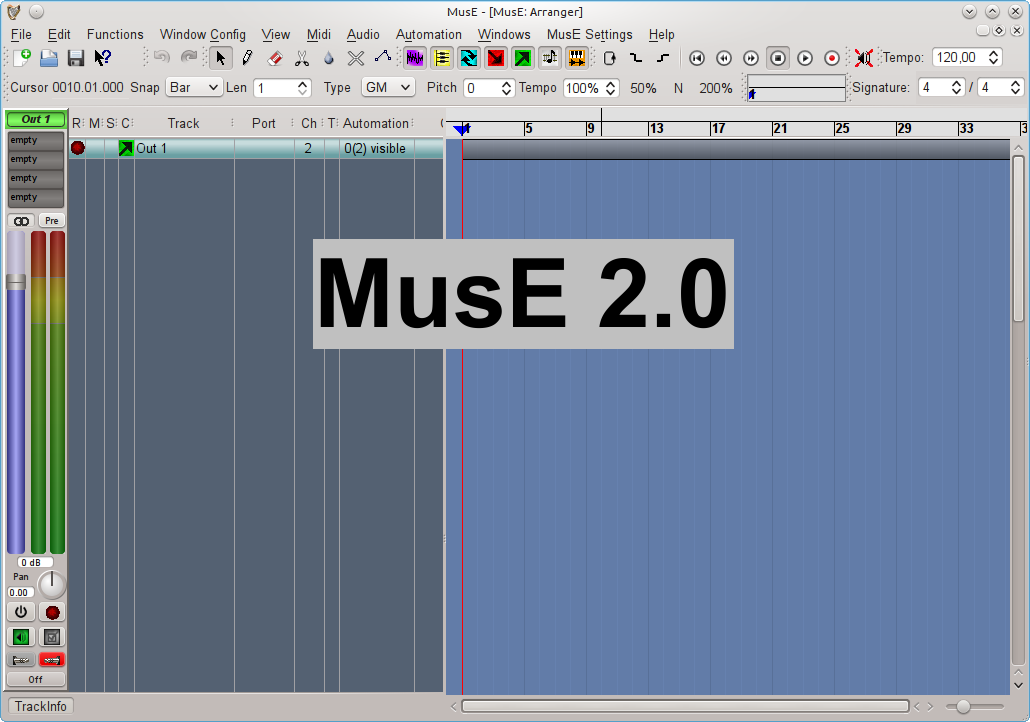
\includegraphics[width=1.0\textwidth]{pics/muse2}
\label{fig:MusE}
\end{figure}
\chapter {What is this?}
You are, if you have printed this document, holding in your hand the
written documentation for the audio and midi sequencer MusE version 2.\\ 
\url{http://www.muse-sequencer.org} is MusE's home on the internet where
everything MusE releated should be possible to find, software, this
documentation, forums, mailing lists, bug reporting, FAQs. If you have
this document but not the software head on over there to find what it's
all about.
\chapter{User's manual}

\section {Introduction}
\subsection {A brief history of computer audio and MusE}
To quickly summarize over a decades open source development: in 1999 Werner
 Schweer released the first version of MusE, muse-0.0.1.tar.gz, in it's first
few releases (actually not few, Werner relentlessly churned out new releases)
MusE was only a midi sequencer. The target was to create a fully fledged
midi sequencer for the Linux operating system. Over the years audio was
added among with other things implemented and sometimes abandoned.
Today MusE is a stable and feature rich music creation environment which
strives to encompass most of the music recording process, creation, editing,
mastering.

\subsection {Definitions}
\key{CTRL} refers to the control key on the keyboard, e.g. \key{CTRL+C}
means to press and hold the control key while pressing the c key. Make sure
you know where you have it so you won't accidentally lose control
(bad jokes are the best jokes, so say we all!).\\
\key{SHIFT} refers to the shift key on the keyboard, see above for usage\\
\key{ALT} refers to the alt key on the keyboard, see above for usage\\
\shell{\$>} is used as a generic definition for a terminal prompt. When the
manual lists a command that shall be typed, the prompt is not part of the
command.\\
Keys are always referred to in bold uppercase, e.g. \key{A}. For instance
\key{SHIFT+A} for the key a pressed together with the shift key.\\
Sometimes terminal examples are written tabbed in with a fixed font to
visualize more closely what something looks like on the screen.
E.g.\\
\hspace*{1cm}\shell{\$> muse2}\\

\subsection {Getting up and running for impatient people}
Install MusE from the repository of your chosen distribution.
To get decent performance start Jack with the following command in a
terminal:\\
\hspace*{1cm}\shell{\$> jackd -d alsa -d hw:0 -p 256}\\
Or, if you prefer, use the launcher utility \textbf{QJackCtl} to get some
help starting Jack.
After this, start MusE from the menu or fire up another terminal and type
\shell{muse2}.\\
If this didn't work out read on for the slighly more complete route for
getting things started.

\subsection {Getting up and running}
\subsubsection {Installation from binaries}
There are several ways to install MusE depending on your situation. The
most convenient way is to install a prepackaged version from your chosen
distribution. The drawback of this is that it may not be the most recent
version, though often there is a more recent package from a private packager.
\subsubsection {Installation from source}
Building MusE from source is not hard, there are a number of prerequistes
that must be met but the actual building should be painless (ha, famous
last words).\\
Please follow the README in the source package and/or read the instructions
on the homepage: \url{http://muse-sequencer.org/index.php/Installation}

\subsubsection {Hardware}
MusE on the Linux platform supports midi through ALSA and Jack-midi and audio
through Jack. For information on what hardware is supported there are some
convenient places to check:
\begin {itemize}
\item Alsa soundcard matrix
\item \url{http://FFADO.org} for firewire devices.
\end {itemize}
Also, as is often a very good approach for Linux and open source, the
various forums available on the internet often contain good information.
Chances are someone has already tried your configuration and/or had your
specific problem and the solution is already written down.
\subsubsection {Launching}
After installation the binary muse2 is installed on the computer. If MusE
was installed from a distribution repository the binary may have a
different name depending on the distribution policies. Most distributions
do however install a menu entry so MusE should be conveniently available
from there.
\subsubsection {Audio preconditions}
In the standard case MusE expects to find and connect to the Jack audio
server \url{http://jackaudio.org}. Make sure jack is installed (if MusE was
installed with a distribution-package Jack will very likely already be
installed) For Jack to run with best performance your system should be
sufficiently tuned to allow it to run with realtime capabilities. The
realtime configuration is configuration of the operating system and roughly
consists of two parts.
\begin {enumerate}
\item By default on most distros only the superuser lets applications setup
realtime capabilities. Please see the APPENDIX for setting up realtime
\item Maximizing performance. A standard linux installation may not able
to reach the performance required by a power user. This requires exchanging
the linux kernel for a so called lowlatency kernel, this is also covered by
the realtime APPENDIX.
\end {enumerate}

\subsubsection {Running MusE}
Find MusE in the menu or open a terminal and enter muse2. A splash screen
should pop up followed by the main application window and you are off!
\shell{\$> muse2}\\
If an error like the screenshot below pops up the Jack audio server is
either not running or started as a different user than what you are trying
to start MusE as.
\begin{figure}[htp]
\centering
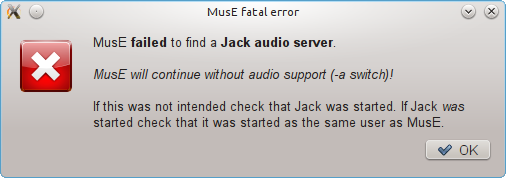
\includegraphics[width=\screenshotwidth]{pics/no_audio}
\caption{Jack server missing}
\label{fig:no_audio}
\end{figure}
\subsubsection {Midi only}
MusE can be started in Midi-only mode where MusE does not have any external
dependencies apart from ALSA midi. In this case start MusE from a terminal:
\shell{\$> muse2 -a}

\subsection {Beginners tutorial}
To get a quick grip of what MusE can achieve please follow this beginners
tutorial.
\subsubsection {Setup}
First off, fire up MusE as was described in the previous chapter, making
sure that the jack audio server is started with sufficient configuration
to allow for audio output without breakup. Also make sure your system can
make sound.
\subsubsection {Soft synth test}
With MusE up and running right click in the Track-pane (see screenshot in
~\ref{Main/Arranger}) and select \menu{Add Synth > MESS > Organ}. A Soft
Synth track called Organ-0 should appear as well as a separate GUI for
the synthesizer.

Now right click once more in the Track-pane and select \menu{Add Midi
Track}. Another track appears called Track-1, you will notice that it is
by default bound to the synth that was just created Organ-0.
\begin{wrapfigure}{r}{0.05\textwidth}

\includegraphics[width=0.05\textwidth]{pics/arrow_tool}
%\hrulefill
\end{wrapfigure}
Now select the drawing tool icon
from the toolbar, alternatively press the shortcut key \key{D}.
Move the mouse over to the arranger canvas as referenced in ~\ref{Main/Arranger}
and point at the midi track, the mouse should have changed to a small pencil.
Draw a Part along the midi track using the mouse. For this exercise it is
not important where or how large the drawn Part is. When you are done double
click on the drawn part. This will open up the Piano Roll editor. To the
left of the Piano Roll there are piano keys in a vertical line, try clicking
on the keys in this virtual keyboard each click should be rewarded with an
organ sound (maybe of questionable quality, a sound nevertheless)
\begin{figure}[htp]
\centering
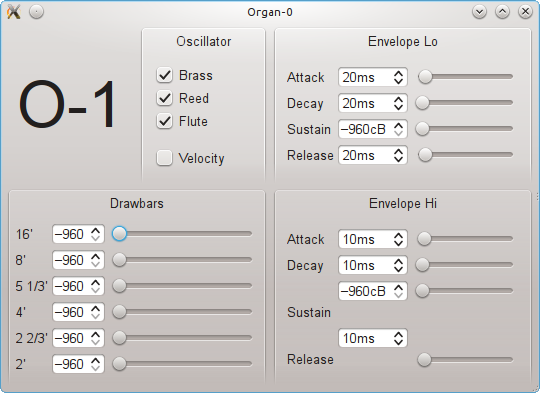
\includegraphics[width=.5\textwidth]{pics/organ_synth}
\caption{Organ synthesizer}
\label{fig:organ_synth}
\end{figure}

\subsubsection {Missing sound}
If you got sound from the previous exercise you can carry on to the next,
or keep reading for further enlightenment in case you come upon trouble
later on. If there are no sound we need to do some fault hunting. First
of, click on Arranger window once more and select the Organ-0 track in the
track-pane.
\begin{figure}[ht]
\centering
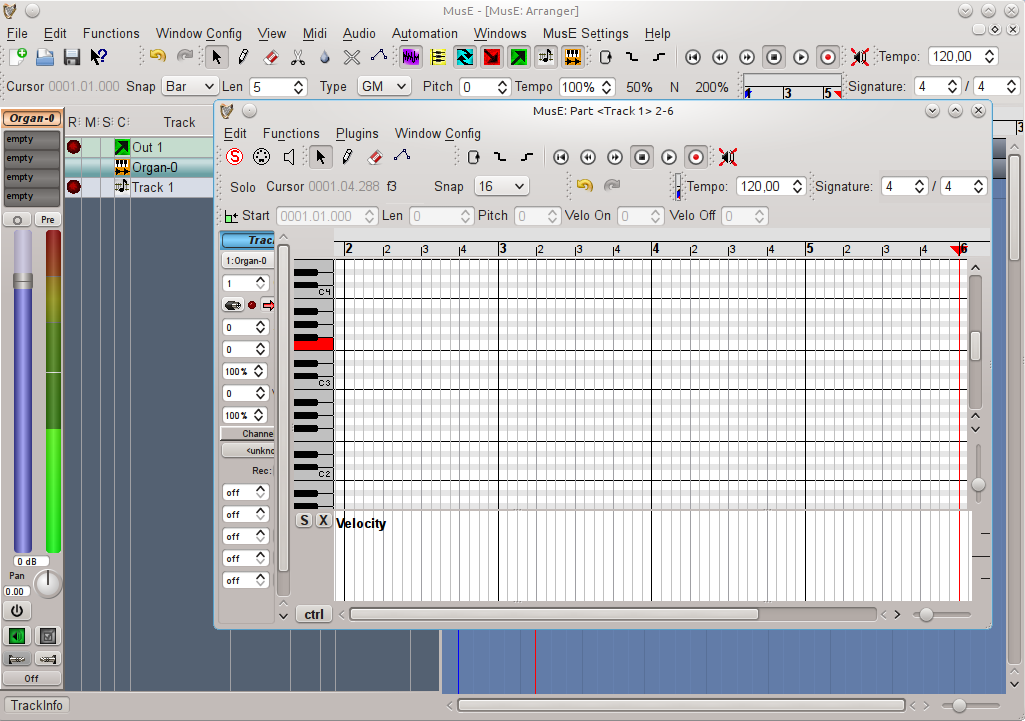
\includegraphics[width=\screenshotwidth]{pics/main_window_with_midi_editor}
\caption{Midi editor view}
\label{fig:Midi editor}
\end{figure}
Now bring back Piano Roll window and align the windows so you
can see the piano keys as well as the Meter on the Mixer Strip (see the
5 Function by function chapter for more information on these windows).
The result should be something like the following:

When pressing one of the keys on virtual Keyboard the Meter on the Mixer
Strip should light up in green to visualize that the Synth is making
sound, if it is not try to trace back your steps and and see if you did
anything differently than described.
Now, if the Meter lights up but there is still no sound we need to to
check the routing between the tracks. Click on the Arranger window again
and select the Out 1 track, this is the predefined output which MusE by
default loads at startup, at the bottom of Mixer Strip there are two
buttons looking like tele- jacks, these bring up the inputs and outputs
of the track, click on the right one, the output and make sure that it is
connected to some valid outputs on your system.
\begin{wrapfigure}{r}{0.25\textwidth}
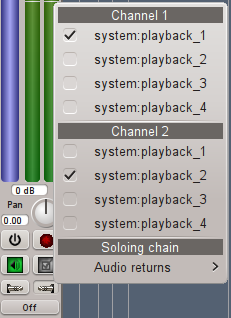
\includegraphics[width=0.25\textwidth]{pics/output_routing}
%\hrulefill
\end{wrapfigure}
Click on the outputs to select them, if you did changes here go back and
try clicking on the Piano Roll keyboard again, hopefully it helped. If there
 still are problems make sure your system actually can make sound through
Jack, this is however getting outside the scope of this manual.\\\\
\textit{This might be the time to bring up the concept of community support.
Open source software could never be what it is without the support given by
individuals on forums and mailinglists, if the information given in this
document is not enough, try googling your problem and/or get in touch with
one of the online forums for MusE or Linux audio in general. See some pointers
in the Support chapter.}

\subsubsection {Recording}                                               %TODO: walkthrough of recording midi
TBD


\section {Basic overview}
In this section we will make a step by step walk-through of all the
different editors, their purpose and what functions they support.

\subsection{Main/Arranger}

\label{Main/Arranger}
\begin{figure}[htp]
\centering
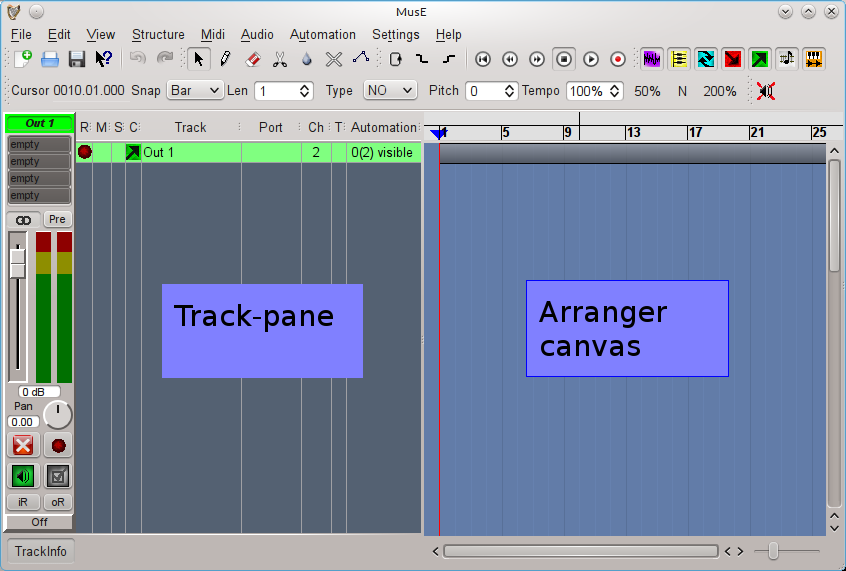
\includegraphics[width=\screenshotwidth]{pics/main_window_annotated}
\caption{MusE main window}
\label{fig:Main Window}
\end{figure}
Above is the main window of MusE, the Arranger, this is what greets you
when launching MusE. The Arranger consists of two main parts, the Track-pane
and the Arranger canvas. The Track-pane lists all currently visible tracks
and the Arranger canvas contains all Parts of the composition. The
screenshot above shows an empty project. Below is MusE with a song in
progress, turns out it wasn't a very good song, but for our purposes it
is fine. In the below screenshot there are a lot of tracks visible in the
Track-pane, each have an icon which indicate it's type, wave-trace, input,
output etcetera, more about that later. In the Arranger canvas a number of
parts are visible, the ones in yellow are in this composition wave files,
the multicolored line are different Parts of a drum track.
\label{Main/Arranger}
\begin{figure}[htp]
\centering
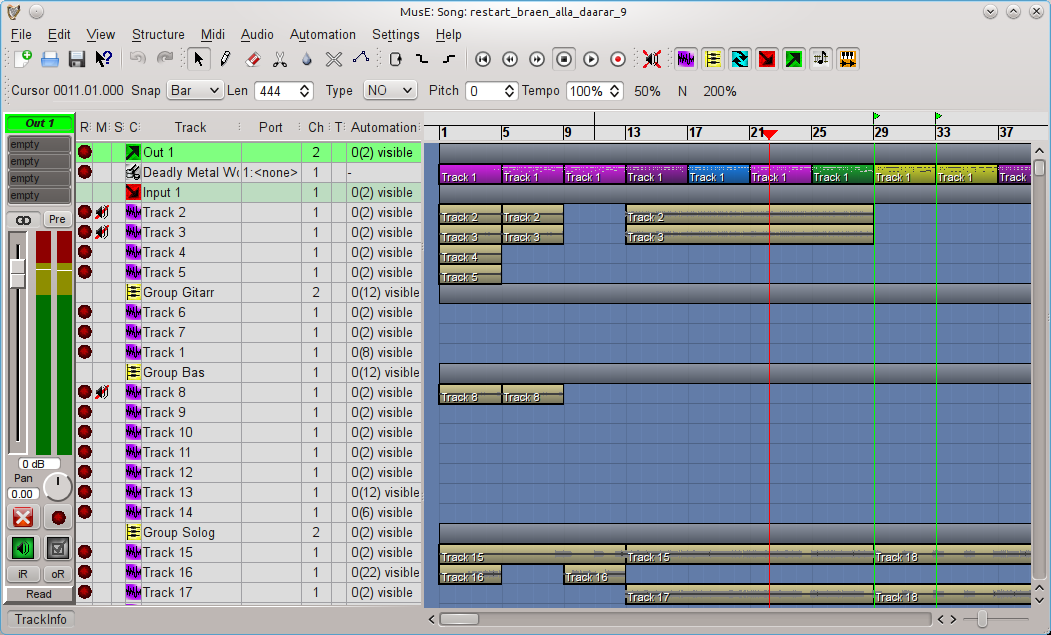
\includegraphics[width=\screenshotwidth]{pics/main_window_with_arrangement}
\caption{MusE main window with arrangement}
\label{fig:Main Window with arrangement}
\end{figure}

\subsection{Mixer}
Choosing \menu{View > Mixer A} or \menu{B} from the menu in the main
window will bring up the mixer as viewed below. The mixer will with all
options enabled show channel strips for all tracks in the current setup,
depending on how far you have gotten this view may become very large,
at which point it may be a good idea to limit what is viewed in the
Mixer. From the view menu all the different kinds of tracks can be
toggled on/off from the mixer. Some may find it a good idea to use the
two mixers A and B setup with different setup and store this in your
song template(s), more about this in the Song Template section. It can
be argued that everything in MusE is a track analogous to the Unix
idiom that everything is a file.
The types of tracks viable in the mixer (and track-pane) are:
\begin{wrapfigure}{r}{0.5\textwidth}

\includegraphics[width=0.5\textwidth]{pics/mixer}
%\hrulefill
\end{wrapfigure}
\begin {itemize}
\item Audio output
\item Audio input
\item Group track
\item Aux track
\item Wave track
\item Synth track
\item Midi track
\end{itemize}


There are also a Midi Track variation called Drum Track, they are 
however not distinguishable from Midi Tracks in the Mixer. Also the 
strips for midi tracks are different in the Mixer than in the 
Track-pane view.


\subsection{Tracks}
MusE arranges your music in \emph{tracks} and \emph{parts}. The following
section shall provice you an overview of how things are done with MusE.
If you are or were a Cubase or Cakewalk user, you will feel familiar with
this. There are
MIDI and drum tracks (which are internally MIDI tracks) which can hold
note data, wave tracks which hold wave data, and several kinds of
audio tracks, synthesizers etc.

\paragraph{MIDI tracks}
MIDI and drum tracks hold MIDI event data. They don't differ much,
except that drum tracks offer a special editor which is more suitable
for drum editing.

\paragraph{Wave tracks}
They hold audio data which can be just played back or be piped through
effect plugin chains. They offer automation for these plugins.

\paragraph{Audio inputs}
These provide the path for your audio data from outside into your
project. Set up the physical audio inputs you want to connect your audio
in track with, and then route them to some wave tracks.

                                                                         % TODO: what are audio outs and auxs?
                                                                         %       someone please write this!
                                                                         
\subsection{Parts}
Tracks are split in parts. These contain MIDI events or wave chunks.
You can copy, clone them, move them around, delete them etc.

\subsection{MIDI ports}
Ports provide an abstraction layer for your MIDI synthesizers (which
can be both software and hardware synthesizers). Port are numbered.
In order to produce sound, each MIDI track is assigned to exactly one
MIDI port, to which the MIDI events are then sent.

In the configuration menu, you must map the port numbers to the actual
synth devices (by selecting ALSA or jack midi ports, or synth plugins).

Try left-clicking on the "Ports" column of some MIDI track. If you
use a soft synth, right-clicking the Ports column of the synth or any
track using the synth lets you launch the synthe's GUI.

\section{Tracks and parts}
\subsection{Tracks}
\paragraph{Creation}
You can create a track by either right-clicking in the arranger's track   % TODO: insert screenshot
list and then adding the desired track, or via the edit menu.

\paragraph{Attributes}                                                    % TODO: this should be a list
Tracks have several attributes.
\subparagraph{Mute} If you click on the \emph{Mute} field (denoted with
a "M" column header), the track gets muted and stops producing sound.
\subparagraph{Solo} The solo button ("S" column header) mutes all other   % TODO: soloing chains etc?
tracks.
\subparagraph{Record} The R column "arms" your track for recording.
When you rec-arm your song and have no tracks rec-armed, you won't be
able to record anything. See also the config option "move rec-arm with    % TODO: reference to rec-arm config option
selection".
\subparagraph{Track name} Double-click and you will see.
\subparagraph{Port} For MIDI tracks, this lets you select the MIDI
port to which the events should be routed. This can be your physical
synthesizer or a software synthesizer. For soft synthes, this is the
port the synth is associated to. For other track types, this is disabled.
\subparagraph{Channel} For MIDI tracks, this is the MIDI channel the
output is sent to. For any kind of audio tracks, this is the number of
channels (mono, stereo).
                                                                          % TODO: what's that "T" column?!
\subparagraph{Automation} For audio tracks, this lets you set up the
automation display in the arranger. Clicking this will provide you with
a popup menu with lots of submenus. The submenus let you select the
color you want to associate with the automation parameter. \emph{Clicking % TODO: this is nonstandard
on a submenu} will select or unselect it, making the automation parameter % TODO: put reference to automation section
shown or hidden.

\subparagraph{Clef} For MIDI tracks, you can specify a clef here. This
only affects the score editor.

\paragraph{The trackinfo side bar}
In the arranger and the part editors, you'll have a trackinfo sidebar
on the left side. You can set up track-type specific things there.

\subsubsection{MIDI tracks}
MIDI parts have no automation settings. However, they support various     % TODO: this will hopefully become wrong soon
controllers, program changes etc.. The MIDI trackinfo sidebar lets you
change program, volume, pan and more. Just editing the value in the
boxes will send an event, but not write it to the track. In order to
write it, you will need to click on the corresponding button ("Vol" for
writing down volume information).

\subsubsection{Old style drum tracks}
These are MIDI tracks as well, but with a few differences. They allow
you to map certain drum sounds with different input notes, and you
can change the output settings of a certain "drum instrument" without
having to alter each single event.

However, they have certain limitations: They only can handle 128 sounds
(even if you have more synthes), they aren't really compatible with
MIDI tracks (you can interchange parts between them, but if you touched
the drum list, you'll get unexpected results), you can't set a program
for the used channel and more.

\subsubsection{New style drum tracks}
Because of these limitations, we introduced the new-style drum tracks.
They're not fully compatible with the old drum tracks, so the old are
still retained. Under "Global Settings", "GUI settings", you can set
up whether you prefer the old or new.

They are handled exactly like plain MIDI tracks (staying compatible with
them), and offer all of the functionality, though in a different way.
They allow you to re-order the drum map efficiently, you can open parts
from multiple drum tracks in \emph{one} drum editor (MusE will separate
the sounds from different tracks according to your settings, see the
"Window Config" menu), and you can set programs as with normal MIDI tracks.

\subsubsection{Audio tracks}
\paragraph{Effect rack}
On the top of the sidebar, there is an effect rack which allows you to
apply various plugins on the audio. For more information on this, refer
to \ref{plugins}.

\paragraph{Controls}
Lorem ipsum % TODO FINDMICH HIER WEITER


\subsection{Parts}
Within MIDI, drum and wave tracks, you can create \emph{parts}. Parts
are chunks of coherent notes or wave data which can be moved around,
copied, cloned and deleted independent from other parts.

Parts are created by selecting the pencil tool and then drawing onto
the right part area in the arranger. You can move them with the arrow
tool, delete them using the \key{DEL} key, and a right-click opens
a popup menu. This menu allows you even more stuff, such as setting
the part's color, saving the part to disk etc.. You can use
\key{CTRL+C} and \key{CTRL+V} for copying and pasting parts.
\key{CTRL+B} pastes the part as a clone. Pressing \key{SHIFT}
additionally provides you a dialog which allows you to paste the part
multiple times and set more stuff.

You can also copy parts with the mouse by moving the part with the mouse
while holding down the \key{CTRL} key.



\section{Plugins and automation} \label{plugins}
There are several kinds of plugins. First, there are audio plugins, which
can be applied to any track handling audio (that is, inputs, outputs,
wave tracks, synth tracks). Plugins can be added by double-clicking
on an entry in the effect rack in the track info pane (which is shown
at the left side of the arranger when the according track is selected).
Right-clicking them offers a self-explanatory popup menu.

\section{Configuration}
\paragraph{Minimum control period}
Plugins can usually process an arbitrarily small (or large) amount of
samples. If some plugin control value changes continously, to provide
ideal listening experience, MusE would need to call the plugin 44100
times a second, asking for one single value at a time. With the minimum
control period setting, the user can force MusE to ask the plugin for
at least N values. Setting this value to 64 would in this situation
make MusE call the plugin $689 = \frac{44100}{64})$ times a second,
asking for 64 values at a time. While doing this will reduce accuracy
of control changes, it may also reduce CPU usage, because calling
the plugin more often, requesting smaller chunks, is more expensive
than calling it seldomly, requesting larger chunks.
\subparagraph{Recommendation}
If you have no performance problems, or if you want to do the final
downmix of your project, set this to a low value. If you're experiencing
performance problems, increasing this value might help.






\chapter{Internals -- how it works}
This chapter explains how MusE is built internally, and is meant
to be an aid for developers wanting to quickly start up with MusE.
For details on \emph{why} stuff is done please refer to the following
chapter.
\section{User controls and automation}
\subsection{Handling user input}
\subsubsection{Plugins and synthesizers}
\paragraph{Overview}
When the user launches a plugin's GUI, either a MusE-window with
the relevant controls is shown, or the native GUI is launched. MusE
will communicate with this native GUI through OSC (Open Sound Control).
The relevant classes are \sym{PluginGui}, \sym{PluginIBase}
(in \file{plugin.h}) and \sym{OscIF} (in \sym{osc.h}).

If the user changes a GUI element, first the corresponding control is
disabled, making MusE not steadily update it through automation
while the user operates it. Then MusE will update the plugin's parameter
value, and also record the new value. When appropriate, the controller
is enabled again.

\paragraph{Processing the input, recording}
Upon operating a slider, \sym{PluginIBase::setParam} is called,
which usually writes the control change into the ringbuffer
\sym{PluginI::{\_}controlFifo}. (\sym{PluginI::apply()},
\sym{DssiSynthIF::getData()} will read this ringbuffer and
do the processing accordingly). Furthermore, \sym{AudioTrack::recordAutomation}
is called, which either directly modifies the controller lists or writes
the change into a "to be recorded"-list (\sym{AudioTrack::{\_}recEvents})
(depending on whether the song is stopped or played).

The \sym{AudioTrack::{\_}recEvents} list consists of \sym{CtrlRecVal}
items (see \file{ctrl.h}), which hold the following data:
\begin{itemize}
\item the frame where the change occurred
\item the value
\item the type, which can be \usym{ARVT{\_}START}, \usym{ARVT{\_}VAL} or \usym{ARVT{\_}STOP}.
      \usym{ARVT{\_}VAL} are written by every \usym{AudioTrack::recordAutomation}
      call, \usym{ARVT{\_}START} and \usym{ARVT{\_}STOP} are generated by
      \sym{AudioTrack::startAutoRecord} and \sym{stopAutoRecord},
      respectively.
\item and the id of the controller which is affected
\end{itemize}
It is processed when the song is stopped. The call path for this is:
\sym{Song::stopRolling} calls \sym{Song::processAutomationEvents}
calls \sym{AudioTrack::processAutomationEvents}.
This function removes the old events from the track's controller list
and replaces them with the new events from \sym{{\_}recEvents}. In
\usym{AUTO{\_}WRITE} mode, just all controller events within the recorded
range are erased; in \usym{AUTO{\_}TOUCH} mode, the \usym{ARVT{\_}START}
and \usym{ARVT{\_}STOP} types of the \sym{CtrlRecVal} events are used
to determine the range(s) which should be wiped.

\paragraph{How it's stored}
Automation data is kept                                                  % this is copied from
in \sym{AudioTrack::{\_}controller}, which is a \sym{CtrlListList},        % "design decisions" -> "automation"
that is, a list of \sym{CtrlList}s, that is, a list of lists of
controller-objects which hold the control points of the automation graph.
The \sym{CtrlList} also stores whether the list is meant discrete
(a new control point results in a value-jump) or continous (a new control
point results in the value slowly sloping to the new value).
Furthermore, it stores a \sym{{\_}curVal} (accessed by \sym{curVal()}),
which holds the currently active value, which can be different from the
actually stored value because of user interaction. This value is also
used when there is no stored automation data.

\sym{AudioTrack::addController} and \sym{removeController} are used        % TODO: swapControllerIDX??
to add/remove whole controller types; the most important functions which
access \sym{{\_}controller} are:
\begin{itemize}
\item \sym{processAutomationEvents}, \sym{recordAutomation},
      \sym{startAutoRecord}, \sym{stopAutoRecord}: see above.
\item \sym{seekPrevACEvent}, \sym{seekNextACEvent}, \sym{eraseACEvent},
      \sym{eraseRangeACEvents}, \sym{addACEvent}, \sym{changeACEvent},
      which do the obvious
\item \sym{pluginCtrlVal}, \sym{setPluginCtrlVal}: the first
      returns the current value according to the \sym{{\_}controller}
      list, the second only sets the \sym{curVal}, but does not
      insert any events.
\end{itemize}

Whenever a \sym{CtrlList} has been manipulated,
\sym{MusEGlobal::song->controllerChange(Track*)} shall be called,
which emits the \sym{MusEGlobal::song->controllerChanged(Track*)}
signal in order to inform any parts of MusE about the change (currently,
only the arranger's part canvas utilizes this).

\paragraph{Enabling and disabling controllers}
Disabling the controller is both dependent from the current automation
mode and from whether the GUI is native or not.
In \usym{AUTO{\_}WRITE} mode, once a slider is touched (for MusE-GUIs) or
once a OSC control change is received (for native GUIs), the control
is disabled until the song is stopped or seeked.

In \usym{AUTO{\_}TOUCH} (and currently (r1492) \usym{AUTO{\_}READ}, but
that's to be fixed) mode, once a MusE-GUI's slider is pressed down, the
corresponding control is disabled. Once the slider is released, the
control is re-enabled again. Checkboxes remain in "disabled" mode,
however they only affect the recorded automation until the last toggle
of the checkbox. (Example: start the song, toggle the checkbox, toggle
it again, wait 10 seconds, stop the song. This will NOT overwrite the
last 10 seconds of automation data, but everything between the first
and the last toggle.). For native GUIs, this is a bit tricky, because
we don't have direct access to the GUI widgets. That is, we have no
way to find out whether the user doesn't touch a control at all, or
whether he has it held down, but just doesn't operate it. The current
behaviour for native GUIs is to behave like in \usym{AUTO{\_}WRITE} mode.

The responsible functions are: \sym{PluginI::oscControl} and
\sym{DssiSynthIF::oscControl} for handling native GUIs,
\sym{PluginI::ctrlPressed} and \sym{ctrlReleased} for MusE
default GUIs and \sym{PluginI::guiParamPressed},
\sym{guiParamReleased}, \sym{guiSliderPressed} and
\sym{guiSliderReleased} for MusE GUIs read from a UI file;
\sym{guiSlider*} obviously handle sliders, while \sym{guiParam*}
handle everything else which is not a slider. They call
\sym{PluginI::enableController} to enable/disable it.

Furthermore, on every song stop or seek, \sym{PluginI::enableAllControllers}
is called, which re-enables all controllers again. The call paths for
this are:
\begin{itemize}
\item For stop: \sym{Song::stopRolling} calls
                \sym{Song::processAutomationEvents} calls
                \sym{Song::clearRecAu{\-}to{\-}ma{\-}tion} calls
                \sym{Track::clearRecAutomation} calls
                \sym{PluginI::enableAllControllers}
\item For seek: \sym{Audio::seek} sends a message ("\sym{G}") to
                \sym{Song::seqSignal} which calls
                \sym{Song::clearRecAutomation} which calls
                \sym{PluginI::enableAllControllers}                
\end{itemize}




\chapter{Design decisions}
\section{Automation}
As of revision 1490, automation is handled in two ways: User-generated
(live) automation data (generated by the user moving sliders while playing)
is fed into \sym{PluginI::{\_}controlFifo}. Automation data is kept
in \sym{AudioTrack::{\_}controller}, which is a \sym{CtrlListList},
that is, a list of \sym{CtrlList}s, that is, a list of lists of
controller-objects which hold the control points of the automation graph.
The \sym{CtrlList} also stores whether the list is meant discrete
(a new control point results in a value-jump) or continous (a new control
point results in the value slowly sloping to the new value).

While \sym{PluginI::{\_}controlFifo} can be queried very quickly and
thus is processed with a very high resolution (only limited by the
minimum control period setting), the automation value are expensive to
query, and are only processed once in an audio \emph{driver} period.
This might lead to noticeable jumps in value.

This could possibly be solved in two ways:
\paragraph{Maintaining a slave control list}
This approach would maintain a fully redundant slave control list,
similar to \sym{PluginI::{\_}controlFifo}. This list must be updated
every time any automation-related thing is changed, and shall contain
every controller change as a tuple of controller number and value.
This could be processed in the same loop as \sym{PluginI::{\_}controlFifo},
making it comfortable to implement; furthermore, it allows to cleanly
offer automation-settings at other places in future (such as storing
automation data in parts or similar).

\paragraph{Holding iterators}
We also could hold a list of iterators of the single \sym{CtrlList}s.
This would also cause low CPU usage, because usually, the iterators only
need to be incremented once. However, it is pretty complex to implement,
because the iterators may become totally wrong (because of a seek in the
song), and we must iterate through a whole list of iterators.

\paragraph{Just use the current data access functions}
By just using the current functions for accessing automation data,
we might get a quick-and-dirty solution, which however wastes way too
much CPU ressources. This is because on \emph{every single frame}, we
need to do a binary search on multiple controller lists.


\chapter{Feature requests}
\section{Per-Part automation and more on automation}                       % by flo
Automation shall be undo-able. Automation shall reside in parts which
are exchangeable, clonable etc (like the MIDI- and Wave-Parts).
Global per-synth/per-audiotrack automation shall also be available, but
this can also be implemented as special case of part automation (one
long part).

\section{Pre-Rendering tracks}
\subsection{The feature}
All tracks shall be able to be "pre-renderable". Pre-rendering shall
be "layered". Pre-rendering shall act like a transparent audio cache:
Audio data is (redundantly) stored, wasting memory in order to save CPU.

That is: Each track owns one or more wave-recordings of the length of
the song. If the user calls "pre-render" on a track, then this track
is played quasi-solo (see below), and the raw audio data is recorded
and stored in the "layer 0" wave recording. If the user has any effects
set up to be applied, then each effect is applied on a different layer
(creating layer 1, layer 2 etc).

This means, that also MIDI and drum tracks can have effects (which
usually only operate on audio, but we HAVE audio data because of this
prerendering).

Furthermore, MusE by default does not send MIDI events to the synthesizers
but instead just plays back the last layer of the prerecording (for
MIDI tracks), or does not pipe the audio data through the whole plugin
chain (causing cpu usage), but instead just plays back the last layer.
The hearable result shall be the same.

Once the user changes any parameter (automation data or plugins for
wave tracks, MIDI events or effect plugin stuff for MIDI tracks),
then MusE shall generate the sound for this particular track in the
"old" way (send MIDI data to synthes, or pipe audio data through plugins).
(So that the user will not even notice that MusE actually pre-renderered
stuff.) Either MusE automatically records this while playback (if possible)
or prompts the user to accordingly set up his cabling and then record
it. Or (temporarily) disables prerecording for this track, falling back
to the plain old way of generating sound.

\emph{Quasi-solo} means: For wave tracks, just solo the track. For MIDI
tracks, mute all tracks which are not on the same synth (channel?),
and mute all \emph{note} events which are not on the quasi-soloed track.
This causes MusE to still play any controller events from different
tracks, because they might have effects on the quasi-soloed track. (You
can have notes on channel 1 on one track and controller stuff on channel
1 on another track; then you would need quasi-solo to get proper results.)

\subsection{Use cases}
\paragraph{Saving CPU}
On slow systems, this is neccessary for songs with lots of, or demanding
(or both) soft synthes / plugins. Even if the synth or plugin is so
demanding that your system is not able to produce sound in real-time,
then with this feature you'll be able to use the synth (this will make
editing pretty laggish, because for a change you need to re-render at
least a part before you can listen to it, but better than being unable
to use the synth at all!)

\paragraph{Exporting as audio project}
Using pre-rendering on all tracks, you easily can export your project
as multi-track audio file (for use with Ardour or similar DAWs).
Just take the last layer of each track, and write the raw audio data
into the file, and you're done. (Maybe we are even able to write down
the raw-raw layer0 audio data plus information about used plugins and
settings etc..?)

\paragraph{Mobile audio workstations}
You might want to work a bit on your audio projects on your notebook
while you're not at home, not having access to your hardware synthesizers.
Using this feature, you could have pre-recorded the stuff in your studio
before, and now can at least fiddle around with the non-hw-synth-dependent
parts of your song, while still having your \emph{full} song with you.

\paragraph{Applying effects on MIDI tracks}
If you have many physical audio inputs, you might already be able to
apply effect chains on MIDI tracks, by wiring the synthes' audio
outputs to your soundcard's inputs, and applying the effects on
dedicated input tracks you have to create. This requires you to have
expensive hardware, and is pretty complicated, because you need one
additional track per MIDI synth.

This feature allows you to apply effects on single MIDI tracks, and not
only on full MIDI synthes, and doesn't require you to be have that
many physical audio inputs (you need to manually replug your synthes,
however).

\subsection{Possible scenarios}
\paragraph{Setting it up}
Create a wave track, MusE will allow you to set or unset prerendering
for every plugin in the plugin rack (recording the actual track is
useless because it would be a plain copy).
Create a MIDI track, MusE will ask you on which physical audio input
your synth is connected. Setting up multiple synthes on one physical 
audio in is allowed, see below.

\paragraph{Pre-rendering stuff}
When the user presses the "pre-render" button, all tracks which have
been changed since their last pre-rendering will be re-rendered.
If you have multiple hardware synthes set up as they were connected
to one physical audio input port, MusE will prompt you to first plug
the proper cable in.

\paragraph{Making changes}
Change a note in a MIDI part, move or delete a part or change automation
parameters. MusE will temporarily disable the pre-rendered information
and instead generate the sound via sending out MIDI events, piping stuff
through effect chains or similar. If you play back the whole song, or
if you manually trigger a re-rendering of a track via the context menu,
MusE will play back the stuff, record it again and re-enable the
pre-rendered information.


\subsection{Extensions}
\paragraph{Automatic discovery of physical audio connections}
The user plugs all (or only some) synthes' audio outs into the available
audio inputs, then runs automatic discovery. This will send MIDI events
to each synthesizer, and look on which audio in there's activity. Then
it will assume that the synthesizer is connected to that particular
audio in. Audio ins which show activity before any MIDI events were
sent are not considered, as they're probably connected to microphones
or other noise-generating non-synthes.

\paragraph{Audio export}
As described in the Use cases, MusE can allow you to export your song
in some multitrack audio format.

\paragraph{Cheap/Faked changes}
For expensive or unavailable synthes, changing the Volume midi controller,
the Pan controller or similar "easy" controllers will not trigger a
complete re-rendering, but instead "fake" the change, by changing
the volume data directly on the recorded wave. This might require some
learning and might even get pretty complicated.

\paragraph{Intelligent re-recording}
For tiny changes, MusE shall only re-render the relevant part. If you
change some MIDI notes, then begin re-recording shortly before the
changes, and end re-recording as soon as the recorded stuff doesn't
differ to much from the stuff coming from the synth. Then properly
blend the old recording with the updated part.



\section{Slotted editors}
Currently, MusE has the pianoroll editor, drum editor, score editor,
then the controller editor which is inside the pianoroll/drum editor.
All these editors have a very similar concept: the "time axis" is
vertical and (almost) linear, they handle parts, and events are
manipulated similarly.

A unified editor shall be created which allows you to combine different
kinds of editors in one window, properly aligned against each other.
These "different kinds of editors" shall be handled as "slots"; one
unified editor window consists of:
\begin{itemize}
\item A menu bar, containing stuff suitable for the complete window,
      which might include window name, MDI-ness etc.
\item A toolbar which contains controls suitable for every single slot.
\item A container with one or more slots; the slots can be scrolled in
      y-direction if there are multipe slots.
\item A time-scrollbar with zoom
\end{itemize}

Each slot contains the following:
\begin{itemize}
\item A menu button, button box or control panel for setting up this
      particular slot. This could contain "note head colors", "show
      a transposing instrument" etc for score edit slots, "event
      rectangle color", "grid size" and "snap to grid" for pianoroll/
      drum editors.
\item The actual canvas
\item A y-direction scroll bar, possibly with zoom control (for
      pianoroll editor)
\end{itemize}

The main window does not show its scroll bar if there is only one slot,
because the slot's scrollbar is sufficient then.

Slots can be added, destroyed, moved around, maybe even merged (if the
slot types allow it); basically, you can compare them with the staves
in the score editor.

The slots shall align against each other, that is, if a score editor
slot displays a key change with lots of accidentials, then all other
slots shall either also display the key change (if they're score slots)
or display a gap. Events which happen at the same time shall be at the
same x-coordinate, regardless which slot they are.

\section{Controller master values}
All controllers (MIDI-controllers and also automation controllers)
shall have one set of "master values" which allow you to set a gain and
a bias. Instead of the actual set value, $\textrm{value} * \textrm{bias}
+ textrm{bias}$ shall be sent to the MIDI device / the plugin. For
controllers like "pan", the unbiased values shall be transformed, that
is, a pan of 64, with $\textrm{bias}=2$ and $\textrm{gain}=0.5$, shall
be transformed to 66 (because 64 is actually 0, while 0 is actually -64).
These values shall be set in the arranger and whereever the actual
controller/automation values can be edited.

\section{Enabled-indicator while recording}
The MusE-plugin-GUIs shall display a small LED displaying whether a
controller is currently enabled or disabled. By clicking this LED, the
enabled state shall be switched.

Furthermore, there shall be a dedicated window which only lets you switch
enabled/disabled states. This will be useful when using external GUIs
or the MIDI-controller-to-automation feature, to re-enable a controller
when in \usym{AUTO{\_}TOUCH} mode.



\section{Linear automation editing}
While holding some modifier key (like shift), operating the MusE-native-
GUI sliders shall only generate control points when clicking and when
releasing the slider. This will result in linear graphs for continous
controllers, and in large steps for discrete controllers (which is in
particular useful for stuff like "which low/high-pass filter type to use").

Maybe make this behaviour default for discrete controllers?



\end{document}

% TODO: song type etc? kill it!
%       song len box: same

% TODO: unified automation and midi ctrls:
%       both shall be editable through the same editors
%       four modes: 1. discrete
%                   2. continous (plus a global and per-port setting for the max rate)
%                   3. switch (not necessarily ON/OFF; signals with color plus text annotation)
%                   4. raw (no graph, instead a box with the value sent out (for "all voices off")
%       they shall be copy-and-pastable, at least between compatible modes
%       they shall be slotted, like pianoroll
%       maybe also "overlapping", like arranger (?)
%       midi recording tries to make out straight lines (like non-ended automation streams)
%       


% new song (in general: load as template) plus "overwrite port config"
% should re-create the default jack devices and autoconnect them.

% what's audio aux for?

% bug in arranger/pcanvas/automation: if a controlpoint is directly on
% a line of another ctrl graph, you can't click it
